\subsubsection{Squared parental income}

This appendix provides a robustness check on the role of squared parental income. We consider the non-logarithmic parental income although standardized.
Table \ref{chap2-tab:rob1-multi1-base} shows the coefficients of the multinomial logistic regression for the probability of being in each first-period occupation.
Table \ref{chap2-tab:rob1-multi2-base} shows the coefficients of the multinomial logistic regression for the probability of being in each second-period occupation.
Table \ref{chap2-tab:rob1-multi3-base} shows the coefficients of the multinomial logistic regression for the probability of being in each second-period occupation according to first-period occupation.

\begin{table}[!htb]
    \centering
    \caption{Probability of being in each occupation in first period (Squared-parental-income robustness check)}
    \label{chap2-tab:rob1-multi1-base}
    \resizebox{\textwidth}{!}{
    \begin{threeparttable}
        \setlength{\tabcolsep}{0pt}
        \begin{tabular}{l D{.}{.}{5.5} D{.}{.}{5.5} D{.}{.}{5.5} D{.}{.}{5.5} D{.}{.}{5.5} D{.}{.}{5.5}}
\toprule
 & \multicolumn{6}{c}{Multinomial logit - Dep. var.: First-period occupation} \\
\cmidrule(lr){2-7}
 & \multicolumn{3}{c}{(1)} & \multicolumn{3}{c}{(2)} \\
\cmidrule(lr){2-4}\cmidrule(lr){5-7}
 & \multicolumn{1}{c}{Low} & \multicolumn{1}{c}{Mid} & \multicolumn{1}{c}{High} & \multicolumn{1}{c}{Low} & \multicolumn{1}{c}{Mid} & \multicolumn{1}{c}{High} \\
\midrule
Intercept                  & 0.08        & 1.39^{***}  & 0.69^{***}  & 0.06        & 1.38^{***}  & 0.66^{***}  \\
                           & (0.07)      & (0.06)      & (0.06)      & (0.07)      & (0.06)      & (0.06)      \\
BCS cohort                 & 0.23^{**}   & 0.12        & 0.76^{***}  & 0.29^{***}  & 0.25^{***}  & 0.90^{***}  \\
                           & (0.10)      & (0.08)      & (0.09)      & (0.11)      & (0.09)      & (0.09)      \\
Female                     & -0.79^{***} & -1.27^{***} & -1.00^{***} & -0.79^{***} & -1.27^{***} & -1.00^{***} \\
                           & (0.09)      & (0.07)      & (0.08)      & (0.09)      & (0.07)      & (0.08)      \\
Female $\times$ BCS        & 0.25^{**}   & -0.01       & -0.07       & 0.25^{**}   & -0.02       & -0.07       \\
                           & (0.12)      & (0.10)      & (0.11)      & (0.12)      & (0.10)      & (0.11)      \\
Par. inc.                  & -0.03       & 0.02        & 0.28^{***}  & -0.04       & 0.02        & 0.26^{***}  \\
                           & (0.04)      & (0.03)      & (0.04)      & (0.04)      & (0.03)      & (0.04)      \\
Par. inc. $\times$ BCS     & 0.09        & 0.20^{***}  & 0.35^{***}  & 0.11        & 0.28^{***}  & 0.46^{***}  \\
                           & (0.06)      & (0.05)      & (0.05)      & (0.07)      & (0.06)      & (0.06)      \\
Par. inc.$^2$              &             &             &             & 0.02        & 0.01        & 0.03        \\
                           &             &             &             & (0.03)      & (0.02)      & (0.02)      \\
Par. inc.$^2$ $\times$ BCS &             &             &             & -0.06       & -0.14^{***} & -0.15^{***} \\
                           &             &             &             & (0.04)      & (0.03)      & (0.03)      \\
\midrule
Num. obs. & \multicolumn{1}{c}{14763} & \multicolumn{1}{c}{14763} & \multicolumn{1}{c}{14763} & \multicolumn{1}{c}{14763} & \multicolumn{1}{c}{14763} & \multicolumn{1}{c}{14763}\\
\bottomrule
\end{tabular}

        \begin{tablenotes}[flushleft]
            \footnotesize{\item\textit{Notes}:
            % Stars and SE
            $^{***}p<0.01$; $^{**}p<0.05$; $^{*}p<0.1$. Standard errors between parentheses. 
            % Referent group
            Male in the NCDS58 cohort is the referent group. 
            % Variables details
            Parental income is standardized at the cohort level and squared parental-income is the square of the standardized parental income.}
        \end{tablenotes}
    \end{threeparttable}
    }
\end{table}

\begin{table}[!htb]
    \centering
    \caption{Probability of being in each occupation in second period (Squared-parental-income robustness check)}
    \label{chap2-tab:rob1-multi2-base}
    \resizebox{\textwidth}{!}{
    \begin{threeparttable}
        \setlength{\tabcolsep}{0pt}
        \begin{tabular}{l D{.}{.}{5.5} D{.}{.}{5.5} D{.}{.}{5.5} D{.}{.}{5.5} D{.}{.}{5.5} D{.}{.}{5.5}}
\toprule
 & \multicolumn{6}{c}{Multinomial logit - Dep. var.: Second-period occupation} \\
\cmidrule(lr){2-7}
 & \multicolumn{3}{c}{(1)} & \multicolumn{3}{c}{(2)} \\
\cmidrule(lr){2-4}\cmidrule(lr){5-7}
 & \multicolumn{1}{c}{Low} & \multicolumn{1}{c}{Mid} & \multicolumn{1}{c}{High} & \multicolumn{1}{c}{Low} & \multicolumn{1}{c}{Mid} & \multicolumn{1}{c}{High} \\
\midrule
Intercept                  & 0.37^{***} & 1.37^{***}  & 1.69^{***}  & 0.45^{***}  & 1.46^{***}  & 1.72^{***}  \\
                           & (0.08)     & (0.07)      & (0.07)      & (0.08)      & (0.07)      & (0.07)      \\
BCS cohort                 & 0.03       & -0.05       & 0.11        & 0.06        & 0.03        & 0.22^{**}   \\
                           & (0.11)     & (0.09)      & (0.09)      & (0.12)      & (0.10)      & (0.10)      \\
Female                     & -0.13      & -1.22^{***} & -1.24^{***} & -0.12       & -1.22^{***} & -1.24^{***} \\
                           & (0.09)     & (0.08)      & (0.08)      & (0.09)      & (0.08)      & (0.08)      \\
Female $\times$ BCS        & -0.04      & -0.12       & 0.17        & -0.05       & -0.13       & 0.17        \\
                           & (0.13)     & (0.12)      & (0.11)      & (0.13)      & (0.12)      & (0.11)      \\
Par. inc.                  & -0.02      & 0.02        & 0.25^{***}  & -0.01       & 0.03        & 0.25^{***}  \\
                           & (0.04)     & (0.04)      & (0.04)      & (0.04)      & (0.04)      & (0.04)      \\
Par. inc. $\times$ BCS     & 0.03       & 0.12^{**}   & 0.28^{***}  & 0.09        & 0.22^{***}  & 0.39^{***}  \\
                           & (0.06)     & (0.06)      & (0.06)      & (0.07)      & (0.06)      & (0.06)      \\
Par. inc.$^2$              &            &             &             & -0.08^{***} & -0.09^{***} & -0.02       \\
                           &            &             &             & (0.03)      & (0.03)      & (0.02)      \\
Par. inc.$^2$ $\times$ BCS &            &             &             & -0.02       & -0.07^{*}   & -0.11^{***} \\
                           &            &             &             & (0.04)      & (0.04)      & (0.03)      \\
\midrule
Num. obs. & \multicolumn{1}{c}{14763} & \multicolumn{1}{c}{14763} & \multicolumn{1}{c}{14763} & \multicolumn{1}{c}{14763} & \multicolumn{1}{c}{14763} & \multicolumn{1}{c}{14763}\\
\bottomrule
\end{tabular}

        \begin{tablenotes}[flushleft]
            \footnotesize{\item\textit{Notes}: 
            % Stars and SE
            $^{***}p<0.01$; $^{**}p<0.05$; $^{*}p<0.1$. Standard errors between parentheses. 
            % Referent group
            Male in the NCDS58 cohort in out-of-work occupation in first period is the referent group. 
            % Variables details
            Parental income is standardized at the cohort level and squared parental-income is the square of the standardized parental income.
            % Explaining bottom panels
            Coefficients in the first bottom panel captures the change in the marginal effect of the first-period occupation with respect to the referent one, i.e. out-of-work. 
            Coefficients in the second bottom panel indicates the change across cohorts in the marginal effect of the first-period occupation.}
        \end{tablenotes}
    \end{threeparttable}
    }
\end{table}

\begin{table}[!htb]
    \centering
    \caption{Probability of being in each occupation in second period (Squared-parental-income robustness check)}
    \label{chap2-tab:rob1-multi3-base}
    \resizebox{\textwidth}{!}{
    \begin{threeparttable}
        \setlength{\tabcolsep}{0pt}
        \begin{tabular}{l D{.}{.}{5.5} D{.}{.}{5.5} D{.}{.}{5.5} D{.}{.}{5.5} D{.}{.}{5.5} D{.}{.}{5.5}}
\toprule
 & \multicolumn{6}{c}{Multinomial logit - Dep. var.: Second-period occupation} \\
\cmidrule(lr){2-7}
 & \multicolumn{3}{c}{(1)} & \multicolumn{3}{c}{(2)} \\
\cmidrule(lr){2-4}\cmidrule(lr){5-7}
 & \multicolumn{1}{c}{Low} & \multicolumn{1}{c}{Mid} & \multicolumn{1}{c}{High} & \multicolumn{1}{c}{Low} & \multicolumn{1}{c}{Mid} & \multicolumn{1}{c}{High} \\
\midrule
Intercept                                                                          & -0.10      & 0.44^{***}  & 0.82^{***}  & -0.03       & 0.52^{***}  & 0.85^{***}  \\
                                                                                   & (0.11)     & (0.10)      & (0.10)      & (0.11)      & (0.11)      & (0.10)      \\
BCS cohort                                                                         & -0.09      & -0.49^{***} & -0.34^{**}  & -0.05       & -0.42^{***} & -0.25^{*}   \\
                                                                                   & (0.15)     & (0.15)      & (0.14)      & (0.16)      & (0.15)      & (0.14)      \\
Female                                                                             & -0.01      & -0.98^{***} & -1.14^{***} & -0.00       & -0.98^{***} & -1.14^{***} \\
                                                                                   & (0.10)     & (0.09)      & (0.09)      & (0.10)      & (0.09)      & (0.09)      \\
Female $\times$ BCS                                                                & -0.10      & -0.09       & 0.27^{**}   & -0.11       & -0.10       & 0.26^{**}   \\
                                                                                   & (0.13)     & (0.12)      & (0.12)      & (0.13)      & (0.12)      & (0.12)      \\
Par. inc.                                                                          & -0.01      & 0.02        & 0.19^{***}  & 0.01        & 0.04        & 0.19^{***}  \\
                                                                                   & (0.04)     & (0.04)      & (0.04)      & (0.04)      & (0.04)      & (0.04)      \\
Par. inc. $\times$ BCS                                                             & 0.03       & 0.09        & 0.18^{***}  & 0.09        & 0.17^{***}  & 0.27^{***}  \\
                                                                                   & (0.07)     & (0.06)      & (0.06)      & (0.07)      & (0.07)      & (0.06)      \\
Par. inc.$^2$                                                                      &            &             &             & -0.08^{***} & -0.09^{***} & -0.03       \\
                                                                                   &            &             &             & (0.03)      & (0.03)      & (0.02)      \\
Par. inc.$^2$ $\times$ BCS                                                         &            &             &             & -0.02       & -0.04       & -0.08^{**}  \\
                                                                                   &            &             &             & (0.04)      & (0.04)      & (0.03)      \\
\midrule\multicolumn{7}{l}{Change with respect to the referent group as first period occupation (Out-of-work)} \\ \midrule
\quad Low-paying                                                                   & 1.00^{***} & 0.31^{**}   & 0.14        & 1.00^{***}  & 0.31^{**}   & 0.14        \\
                                                                                   & (0.12)     & (0.13)      & (0.13)      & (0.12)      & (0.13)      & (0.13)      \\
\quad Middling                                                                     & 0.50^{***} & 1.47^{***}  & 0.81^{***}  & 0.51^{***}  & 1.48^{***}  & 0.82^{***}  \\
                                                                                   & (0.11)     & (0.10)      & (0.10)      & (0.11)      & (0.10)      & (0.10)      \\
\quad High-paying                                                                  & 0.06       & 0.52^{***}  & 1.94^{***}  & 0.07        & 0.53^{***}  & 1.95^{***}  \\
                                                                                   & (0.14)     & (0.14)      & (0.12)      & (0.14)      & (0.14)      & (0.12)      \\
\midrule\multicolumn{7}{l}{Change between cohorts} \\ \midrule
\quad Low. $\times$ BCS                                                            & 0.47^{***} & 0.66^{***}  & 0.56^{***}  & 0.46^{***}  & 0.65^{***}  & 0.55^{***}  \\
                                                                                   & (0.17)     & (0.19)      & (0.18)      & (0.17)      & (0.19)      & (0.18)      \\
\quad Mid. $\times$ BCS                                                            & 0.03       & 0.57^{***}  & 0.27^{*}    & 0.01        & 0.54^{***}  & 0.25^{*}    \\
                                                                                   & (0.15)     & (0.15)      & (0.15)      & (0.15)      & (0.15)      & (0.15)      \\
\quad High. $\times$ BCS                                                           & 0.19       & 0.39^{**}   & 0.18        & 0.17        & 0.37^{**}   & 0.16        \\
                                                                                   & (0.19)     & (0.19)      & (0.16)      & (0.19)      & (0.19)      & (0.16)      \\
\midrule
Num. obs. & \multicolumn{1}{c}{14763} & \multicolumn{1}{c}{14763} & \multicolumn{1}{c}{14763} & \multicolumn{1}{c}{14763} & \multicolumn{1}{c}{14763} & \multicolumn{1}{c}{14763}\\
\bottomrule
\end{tabular}

        \begin{tablenotes}[flushleft]
            \footnotesize{\item\textit{Notes}: 
            % Stars and SE
            $^{***}p<0.01$; $^{**}p<0.05$; $^{*}p<0.1$. Standard errors between parentheses. 
            % Referent group
            Male in the NCDS58 cohort in out-of-work occupation in first period is the referent group. 
            % Variables details
            Parental income is standardized at the cohort level and squared parental-income is the square of the standardized parental income.
            % Explaining bottom panels
            Coefficients in the first bottom panel captures the change in the marginal effect of the first-period occupation with respect to the referent one, i.e. out-of-work. 
            Coefficients in the second bottom panel indicates the change across cohorts in the marginal effect of the first-period occupation.}
        \end{tablenotes}
    \end{threeparttable}
    }
\end{table}

\clearpage
\subsubsection{First-period age}

This appendix provides a robustness check about the difference in terms of age in the first period between both cohorts.
Tables \ref{chap2-tab:rob2-multi1-base} and \ref{chap2-tab:rob2-multi3-base} show the coefficients of the multinomial logistic regressions for the probability of being in each occupation in first and second periods, when both cohorts are either 23 or 26 years old and compare them to their respective baseline estimates from Tables \ref{chap2-tab:occ-multi1-base} and \ref{chap2-tab:occ-multi23-base}.

% \clearpage

\begin{landscape}
\begin{table}[!htb]
    \centering
    \caption{Probability of being in each occupation in first period (First-period age robustness check)}
    \label{chap2-tab:rob2-multi1-base}
    % \resizebox*{!}{\dimexpr\textheight-2\baselineskip\relax}{
    % \resizebox{\textwidth}{!}{
    \begin{threeparttable}
        \setlength{\tabcolsep}{-2pt}
        \begin{tabular}{l D{.}{.}{5.5} D{.}{.}{5.5} D{.}{.}{5.5} D{.}{.}{5.5} D{.}{.}{5.5} D{.}{.}{5.5} D{.}{.}{5.5} D{.}{.}{5.5} D{.}{.}{5.5}}
\toprule
 & \multicolumn{9}{c}{Multinomial logit - Dep. var.: First-period occupation} \\
\cmidrule(lr){2-10}
 & \multicolumn{3}{c}{(Base)} & \multicolumn{3}{c}{(Age 23)} & \multicolumn{3}{c}{(Age 26)} \\
\cmidrule(lr){2-4}\cmidrule(lr){5-7}\cmidrule(lr){8-10}
 & \multicolumn{1}{c}{Low} & \multicolumn{1}{c}{Mid} & \multicolumn{1}{c}{High} & \multicolumn{1}{c}{Low} & \multicolumn{1}{c}{Mid} & \multicolumn{1}{c}{High} & \multicolumn{1}{c}{Low} & \multicolumn{1}{c}{Mid} & \multicolumn{1}{c}{High} \\
\midrule
Intercept              & 0.08        & 1.39^{***}  & 0.69^{***}  & 0.08        & 1.39^{***}  & 0.69^{***}  & 0.31^{***}  & 1.62^{***}  & 1.13^{***}  \\
                       & (0.07)      & (0.06)      & (0.06)      & (0.07)      & (0.06)      & (0.06)      & (0.08)      & (0.06)      & (0.07)      \\
BCS cohort             & 0.24^{**}   & 0.12        & 0.75^{***}  & -0.27^{***} & -0.37^{***} & -0.11       & 0.01        & -0.11       & 0.31^{***}  \\
                       & (0.10)      & (0.08)      & (0.09)      & (0.09)      & (0.07)      & (0.08)      & (0.10)      & (0.09)      & (0.09)      \\
Female                 & -0.79^{***} & -1.27^{***} & -0.99^{***} & -0.79^{***} & -1.27^{***} & -0.99^{***} & -1.17^{***} & -1.88^{***} & -1.59^{***} \\
                       & (0.09)      & (0.07)      & (0.08)      & (0.09)      & (0.07)      & (0.08)      & (0.09)      & (0.08)      & (0.08)      \\
Female $\times$ BCS    & 0.25^{**}   & -0.02       & -0.08       & 0.65^{***}  & 0.49^{***}  & 0.48^{***}  & 0.63^{***}  & 0.60^{***}  & 0.52^{***}  \\
                       & (0.12)      & (0.10)      & (0.11)      & (0.12)      & (0.10)      & (0.10)      & (0.13)      & (0.11)      & (0.11)      \\
Par. inc.              & -0.03       & -0.00       & 0.21^{***}  & -0.03       & -0.00       & 0.21^{***}  & -0.02       & 0.03        & 0.25^{***}  \\
                       & (0.04)      & (0.03)      & (0.04)      & (0.04)      & (0.03)      & (0.04)      & (0.04)      & (0.03)      & (0.04)      \\
Par. inc. $\times$ BCS & 0.10^{*}    & 0.22^{***}  & 0.41^{***}  & -0.07       & 0.04        & 0.16^{***}  & 0.09        & 0.19^{***}  & 0.37^{***}  \\
                       & (0.06)      & (0.05)      & (0.05)      & (0.05)      & (0.05)      & (0.05)      & (0.06)      & (0.05)      & (0.05)      \\
\midrule
Num. obs. & \multicolumn{1}{c}{14763} & \multicolumn{1}{c}{14763} & \multicolumn{1}{c}{14763} & \multicolumn{1}{c}{14522} & \multicolumn{1}{c}{14522} & \multicolumn{1}{c}{14522} & \multicolumn{1}{c}{14710} & \multicolumn{1}{c}{14710} & \multicolumn{1}{c}{14710}\\
\bottomrule
\end{tabular}

        \begin{tablenotes}[flushleft]
            \footnotesize{\item\textit{Notes}: 
            % Stars and SE
            $^{***}p<0.01$; $^{**}p<0.05$; $^{*}p<0.1$. Standard errors between parentheses. 
            % Baseline outcome
            Out-of-work occupation in second period is the base outcome of the multinomial logistic regression.
            % Referent group
            Male in the NCDS58 cohort in out-of-work occupation in first period is the referent group. 
            % Variables details
            Parental income in logarithm and then standardized at the cohort level. 
            % Explaining bottom panels
            Coefficients in the first bottom panel captures the change in the marginal effect of the first-period occupation with respect to the referent one, i.e. out-of-work. Coefficients in the second bottom panel indicates the change across cohorts in the marginal effect of the first-period occupation.
            % Columns
            Columns (Base) correspond to the baseline estimate from table \ref{chap2-tab:occ-multi1-base}. Columns (Age 23) estimate the same regression with first-period occupation at the age of 23 for both cohorts. Columns (Age 26) estimate the same regression with first-period occupation at the age of 26 for both cohorts.}
        \end{tablenotes}
    \end{threeparttable}
    % }
\end{table}
\end{landscape}

% \clearpage

% \begin{landscape}
\begin{table}[!htb]
    \centering
    \caption{Probability of being in each occupation in second period (First-period age robustness check)}
    \label{chap2-tab:rob2-multi3-base}
    % \resizebox*{!}{\dimexpr\textheight-2\baselineskip\relax}{
    \resizebox{\textwidth}{!}{
    \begin{threeparttable}
        \setlength{\tabcolsep}{-4pt}
        \begin{tabular}{l D{.}{.}{5.5} D{.}{.}{5.5} D{.}{.}{5.5} D{.}{.}{5.5} D{.}{.}{5.5} D{.}{.}{5.5} D{.}{.}{5.5} D{.}{.}{5.5} D{.}{.}{5.5}}
\toprule
 & \multicolumn{9}{c}{Multinomial logit - Dep. var.: Second-period occupation} \\
\cmidrule(lr){2-10}
 & \multicolumn{3}{c}{(Base)} & \multicolumn{3}{c}{(Age 23)} & \multicolumn{3}{c}{(Age 26)} \\
\cmidrule(lr){2-4}\cmidrule(lr){5-7}\cmidrule(lr){8-10}
 & \multicolumn{1}{c}{Low} & \multicolumn{1}{c}{Mid} & \multicolumn{1}{c}{High} & \multicolumn{1}{c}{Low} & \multicolumn{1}{c}{Mid} & \multicolumn{1}{c}{High} & \multicolumn{1}{c}{Low} & \multicolumn{1}{c}{Mid} & \multicolumn{1}{c}{High} \\
\midrule
Intercept                                                                          & -0.10      & 0.44^{***}  & 0.81^{***}  & -0.10      & 0.44^{***}  & 0.81^{***}  & -0.02      & 0.50^{***}  & 0.52^{***}  \\
                                                                                   & (0.11)     & (0.10)      & (0.10)      & (0.11)     & (0.10)      & (0.10)      & (0.11)     & (0.10)      & (0.10)      \\
BCS cohort                                                                         & -0.07      & -0.46^{***} & -0.32^{**}  & -0.10      & -0.30^{**}  & 0.36^{***}  & -0.15      & -0.52^{***} & -0.03       \\
                                                                                   & (0.15)     & (0.15)      & (0.14)      & (0.15)     & (0.15)      & (0.13)      & (0.15)     & (0.15)      & (0.14)      \\
Female                                                                             & -0.01      & -0.98^{***} & -1.13^{***} & -0.01      & -0.98^{***} & -1.13^{***} & -0.01      & -0.88^{***} & -0.94^{***} \\
                                                                                   & (0.10)     & (0.09)      & (0.09)      & (0.10)     & (0.09)      & (0.09)      & (0.10)     & (0.09)      & (0.09)      \\
Female $\times$ BCS                                                                & -0.11      & -0.09       & 0.25^{**}   & -0.14      & -0.20       & 0.10        & -0.11      & -0.19       & 0.07        \\
                                                                                   & (0.13)     & (0.12)      & (0.12)      & (0.13)     & (0.12)      & (0.12)      & (0.13)     & (0.12)      & (0.12)      \\
Par. inc.                                                                          & 0.02       & 0.05        & 0.14^{***}  & 0.02       & 0.05        & 0.14^{***}  & 0.03       & 0.05        & 0.13^{***}  \\
                                                                                   & (0.04)     & (0.04)      & (0.04)      & (0.04)     & (0.04)      & (0.04)      & (0.04)     & (0.04)      & (0.04)      \\
Par. inc. $\times$ BCS                                                             & 0.05       & 0.11^{**}   & 0.25^{***}  & 0.06       & 0.13^{**}   & 0.34^{***}  & 0.04       & 0.11^{*}    & 0.26^{***}  \\
                                                                                   & (0.06)     & (0.06)      & (0.05)      & (0.06)     & (0.06)      & (0.05)      & (0.06)     & (0.06)      & (0.05)      \\
\midrule\multicolumn{10}{l}{Change with respect to the referent group as first period occupation (Out-of-work)} \\ \midrule
\quad Low-paying                                                                   & 1.00^{***} & 0.31^{**}   & 0.14        & 1.00^{***} & 0.31^{**}   & 0.14        & 1.03^{***} & 0.30^{**}   & 0.40^{***}  \\
                                                                                   & (0.12)     & (0.13)      & (0.13)      & (0.12)     & (0.13)      & (0.13)      & (0.12)     & (0.13)      & (0.13)      \\
\quad Middling                                                                     & 0.50^{***} & 1.47^{***}  & 0.82^{***}  & 0.50^{***} & 1.47^{***}  & 0.82^{***}  & 0.36^{***} & 1.44^{***}  & 1.00^{***}  \\
                                                                                   & (0.11)     & (0.10)      & (0.10)      & (0.11)     & (0.10)      & (0.10)      & (0.11)     & (0.11)      & (0.11)      \\
\quad High-paying                                                                  & 0.06       & 0.52^{***}  & 1.96^{***}  & 0.06       & 0.52^{***}  & 1.96^{***}  & -0.06      & 0.23^{*}    & 2.17^{***}  \\
                                                                                   & (0.14)     & (0.14)      & (0.12)      & (0.14)     & (0.14)      & (0.12)      & (0.14)     & (0.14)      & (0.12)      \\
\midrule\multicolumn{10}{l}{Change between cohorts} \\ \midrule
\quad Low. $\times$ BCS                                                            & 0.47^{***} & 0.66^{***}  & 0.55^{***}  & 0.39^{**}  & 0.55^{***}  & 0.11        & 0.44^{***} & 0.67^{***}  & 0.29        \\
                                                                                   & (0.17)     & (0.19)      & (0.18)      & (0.17)     & (0.19)      & (0.17)      & (0.17)     & (0.19)      & (0.18)      \\
\quad Mid. $\times$ BCS                                                            & 0.02       & 0.55^{***}  & 0.25^{*}    & 0.13       & 0.39^{***}  & -0.31^{**}  & 0.16       & 0.59^{***}  & 0.06        \\
                                                                                   & (0.15)     & (0.15)      & (0.15)      & (0.15)     & (0.15)      & (0.14)      & (0.16)     & (0.15)      & (0.15)      \\
\quad High. $\times$ BCS                                                           & 0.17       & 0.37^{**}   & 0.15        & 0.48^{**}  & 0.43^{**}   & -0.38^{**}  & 0.29       & 0.66^{***}  & -0.06       \\
                                                                                   & (0.19)     & (0.19)      & (0.16)      & (0.19)     & (0.19)      & (0.16)      & (0.18)     & (0.19)      & (0.16)      \\
\midrule
Num. obs. & \multicolumn{1}{c}{14763} & \multicolumn{1}{c}{14763} & \multicolumn{1}{c}{14763} & \multicolumn{1}{c}{14522} & \multicolumn{1}{c}{14522} & \multicolumn{1}{c}{14522} & \multicolumn{1}{c}{14710} & \multicolumn{1}{c}{14710} & \multicolumn{1}{c}{14710}\\
\bottomrule
\end{tabular}

        \begin{tablenotes}[flushleft]
            \footnotesize{\item\textit{Notes}: 
            % Stars and SE
            $^{***}p<0.01$; $^{**}p<0.05$; $^{*}p<0.1$. Standard errors between parentheses. 
            % Baseline outcome
            Out-of-work occupation in second period is the base outcome of the multinomial logistic regression.
            % Referent group
            Male in the NCDS58 cohort in out-of-work occupation in first period is the referent group. 
            % Variables details
            Parental income in logarithm and then standardized at the cohort level. 
            % Columns
            Columns (Base) correspond to the baseline estimate from columns (2) in table \ref{chap2-tab:occ-multi23-base}. Columns (Age 23) estimate the same regression with first-period occupation at the age of 23 for both cohorts. Columns (Age 26) estimate the same regression with first-period occupation at the age of 26 for both cohorts.}
        \end{tablenotes}
    \end{threeparttable}
    }
\end{table}
% \end{landscape}

\clearpage
\subsubsection{Business cycles}

This appendix provides a robustness check about business cycles. One might be concern by the fact that we measure the individual's employment situation in given years, namely, 1981 and 2000 for the NCDS58 and 1996 and 2012 for the BCS70. Since business cycles can affect employment status, especially in recessions, our comparisons may be biased if we are considering occupational outcomes at different points in the business cycle. 

Figure \ref{chap2-fig:gdp-growth} displays the quarterly UK GDP growth rate between 1975 and 2015. We identify three periods of recessions which can be threats to our analysis: the Early 1980s recession (from 1979Q1 to 1981Q1), the Early 1990s recession (from 1990Q3 to 1992Q2), and the Great Recession (from 2008Q2 to 2009Q2). 
\begin{figure}[!htb]
    \centering
    \caption{UK GDP growth rate (1975-2015)}
    \label{chap2-fig:gdp-growth}
    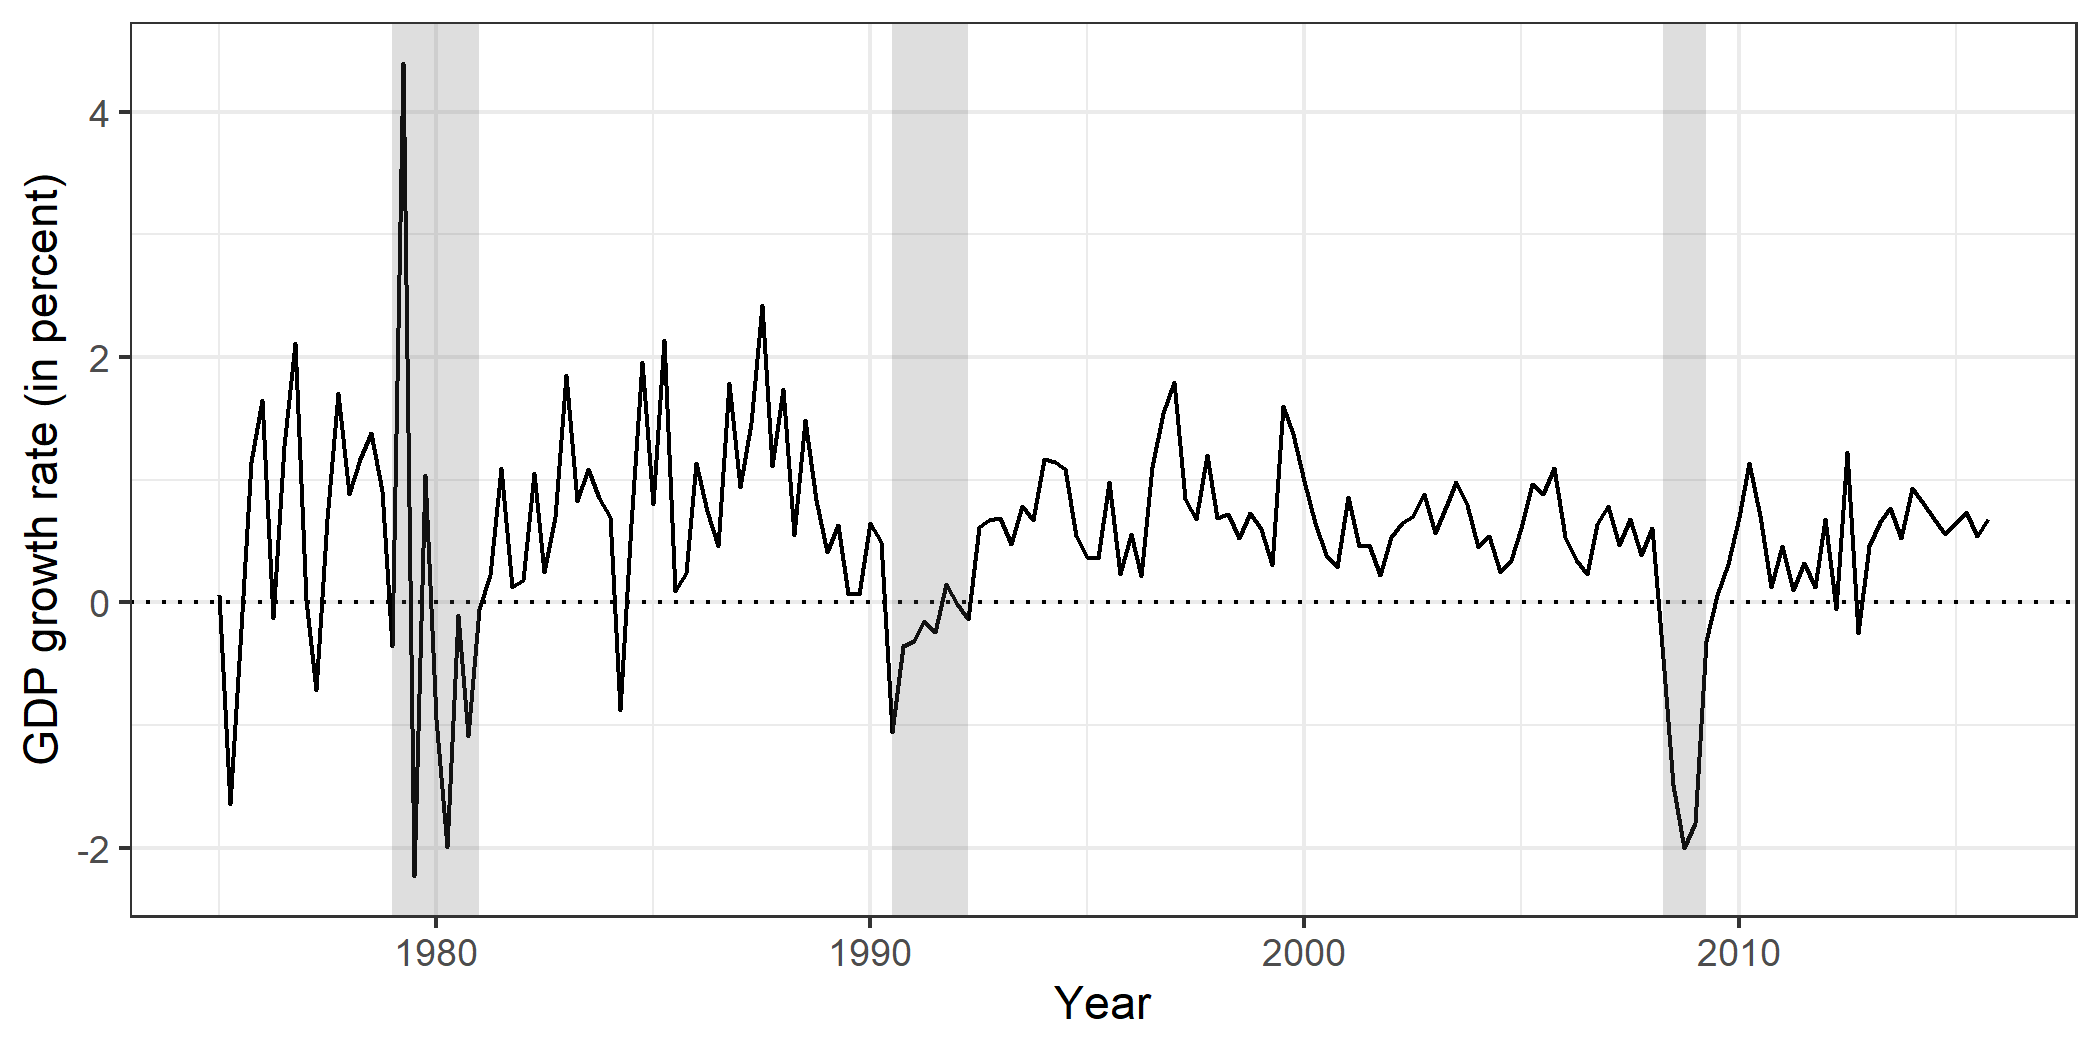
\includegraphics[width=\linewidth]{chap2/graphic/gdp-growth.png}
    \vspace{-3em}
	\justify\singlespacing\footnotesize{\textit{Notes:} This figure presents the quarterly GDP growth rate in the UK from 1975 to 2015. GDP is measured in chained volume and seasonally adjusted. Data are from the Office for National Statistics \href{https://www.ons.gov.uk/economy/grossdomesticproductgdp/timeseries/abmi/pn2}{Office for National Statistics}. Highlighted periods refer to recession periods in the UK.}
\end{figure}

Figure \ref{chap2-fig:lfs-national-cycle} presents the occupational dynamics for individuals born in the same years as our two cohorts using data from the LFS. Our estimates of probabilities for first-period and second-period occupations are performed at the start and the end of those curves. For the NCDS58, we consider their first period at age 23, hence in year 1981, which lies in a the Early 1980s recession. For other periods, they do not seem to be affected by business cycle dynamics as they follow the expected steady trends.
\begin{figure}[!htb]
    \centering
    \caption{LFS occupational dynamics over both cohort lifecycle}
    \label{chap2-fig:lfs-national-cycle}
    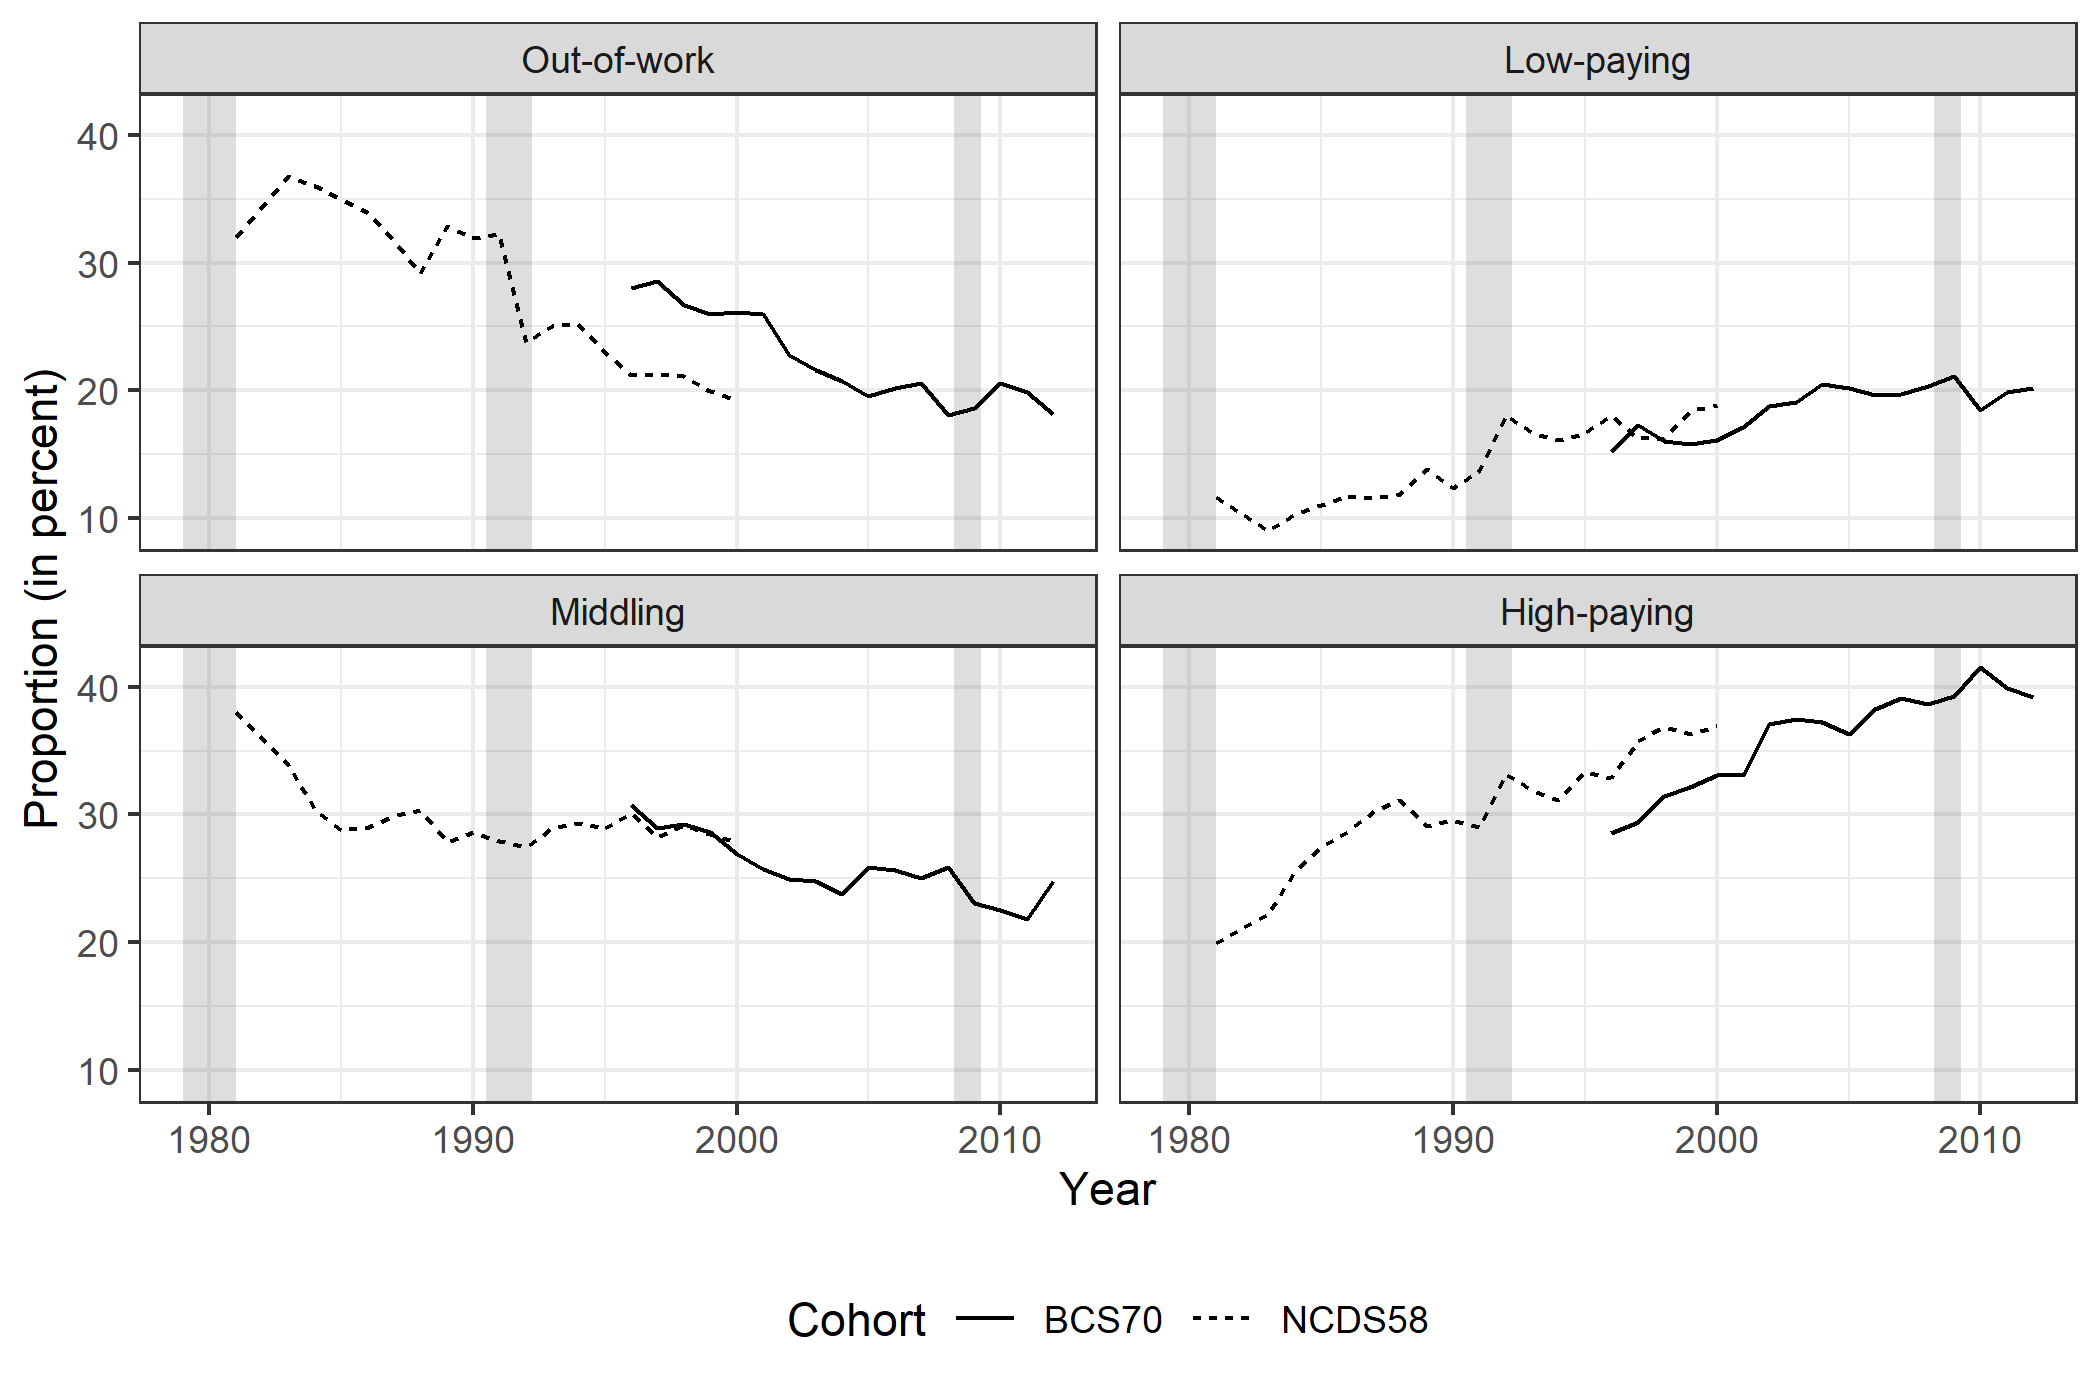
\includegraphics[width=\linewidth]{chap2/graphic/lfs-national-cycle.png}
    \vspace{-3em}
	\justify\singlespacing\footnotesize{\textit{Notes:} This figure presents the job polarization at the national level using the Labour Force Survey (LFS) data from 1981 to 2012. Curves represent the share of individuals in out-of-work, low-paying, middling, and high-paying occupations from the LFS for individuals born in the same year as the BCS70 and NCDS58 cohorts. Highlighted periods refer to recession periods in the UK.}
\end{figure}
The concern about the age of 23 as first period for the NCDS58 cohort can be addressed by looking at tables \ref{chap2-tab:rob2-multi1-base} and \ref{chap2-tab:rob2-multi3-base}. In those tables, we provide estimates of our main regressions when both cohorts are either 23 or 26 years old and show that our results are not driven by first-period age difference. The older cohort is age 26 in 1984 which does not lie in the Early 1980s recession.